% Tiga bukti (3 angka kunci deck): hemat, identik, jalan live.
\documentclass[border=4pt]{standalone}
% Gaya bersama gambar deck Demo Day (dipakai semua gambar/*.tex standalone).
\usepackage{amssymb}
\usepackage{fontspec}
\setmainfont{DejaVu Sans Condensed}
\setsansfont{DejaVu Sans Condensed}
\newfontfamily\judulfont{DejaVu Sans}[BoldFont={DejaVu Sans Bold}, Ligatures=TeX]
\usepackage{tikz,pgfplots}
\pgfplotsset{compat=1.18, every axis/.append style={/pgf/number format/assume math mode=true, /pgf/number format/use comma, /pgf/number format/1000 sep={.}}}
\usetikzlibrary{positioning,arrows.meta,calc,shapes.geometric,fit,backgrounds}
\definecolor{gelap}{HTML}{15242B}
\definecolor{teal}{HTML}{285052}
\definecolor{amber}{HTML}{E8A317}
\definecolor{muda}{HTML}{DCE8E8}
\definecolor{abu}{HTML}{8A9499}
\definecolor{teks}{HTML}{1E2B30}
\definecolor{hijau}{HTML}{2F7D5B}
\definecolor{merah}{HTML}{A33A2A}
\color{teks}
\tikzset{
  ubin/.style={fill=muda, rounded corners=5pt, align=center, inner sep=6pt},
  inti/.style={ubin, fill=gelap, text=white},
  panah/.style={-{Stealth[length=3mm]}, line width=1.3pt, draw=amber},
  panahabu/.style={-{Stealth[length=2.5mm]}, line width=1pt, draw=abu},
  judulubin/.style={font=\judulfont\bfseries},
}
% Dibuat otomatis oleh buat_aset.py dari ml/results/energi_harian.json; jangan diedit manual.
\newcommand{\energiTurbin}{270}
\newcommand{\energiQa}{187}
\newcommand{\energiQb}{377}
\newcommand{\hariEnergi}{140}
\newcommand{\raspiWh}{71}
\newcommand{\chipWh}{4,1}
\newcommand{\raspiPersen}{26}
\newcommand{\chipPersen}{1,5}
\newcommand{\raspiPersenA}{19}
\newcommand{\raspiPersenB}{38}
\newcommand{\raspiPersenNum}{26.3}
\newcommand{\chipPersenNum}{1.5}
\newcommand{\hematKwh}{24}
\newcommand{\kaliHemat}{17}
\newcommand{\jRaspi}{182}
\newcommand{\jChip}{10,4}
\newcommand{\periodeEnergi}{2026-03-31--2026-10-20}

\AtBeginDocument{\hyphenpenalty=10000 \exhyphenpenalty=10000}

\begin{document}
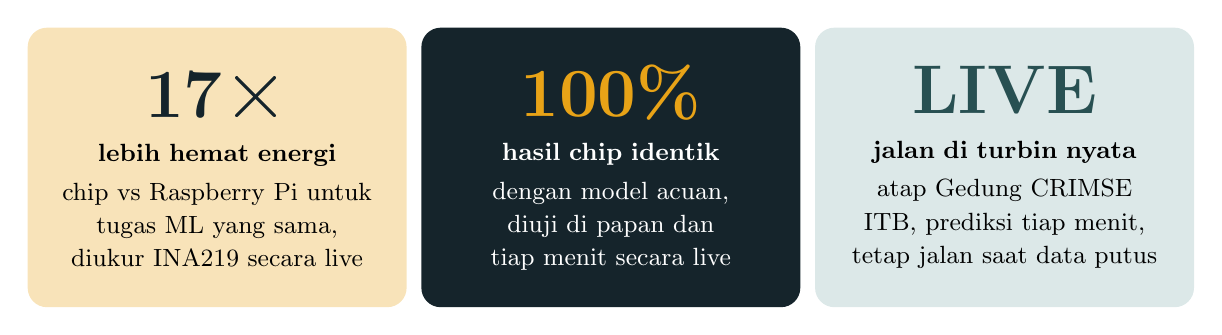
\begin{tikzpicture}[font=\fontsize{9.5}{12}\selectfont,
  bukti/.style={rounded corners=7pt, text width=4.25cm, minimum height=3.55cm, align=center, inner sep=8pt, anchor=north west}]
  \node[bukti, fill=amber!30] at (0,0) {{\judulfont\bfseries\fontsize{30}{32}\selectfont\color{gelap}\kaliHemat\texttimes}\\[4pt]
    {\bfseries lebih hemat energi}\\[2pt]chip vs Raspberry Pi untuk tugas ML yang sama, diukur INA219 secara live};
  \node[bukti, fill=gelap, text=white] at (5.0,0) {{\judulfont\bfseries\fontsize{30}{32}\selectfont\color{amber}100\%}\\[4pt]
    {\bfseries hasil chip identik}\\[2pt]dengan model acuan, diuji di papan dan tiap menit secara live};
  \node[bukti, fill=muda] at (10.0,0) {{\judulfont\bfseries\fontsize{30}{32}\selectfont\color{teal}LIVE}\\[4pt]
    {\bfseries jalan di turbin nyata}\\[2pt]atap Gedung CRIMSE ITB, prediksi tiap menit, tetap jalan saat data putus};
\end{tikzpicture}
\end{document}
